%!TEX root = ../../thesis.tex
\section{Locking}
\label{sync-locking}

\begin{figure}[htb]
  \centerline{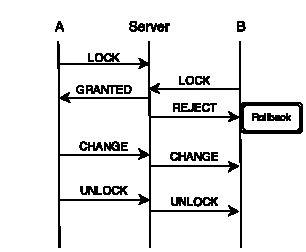
\includegraphics[width=0.65\linewidth]{images/Locking.pdf}}
  \caption[Communication in a locking algorithm]{Communication in a locking algorithm}
  \label{fig:Locking}
\end{figure}

Locking algorithms, often also referred to as `pessimistic' algorithms, define a system in which only one user is allowed to edit a document with simultaneous edits being forbidden \cite[p. 2]{fraser2009differential}. When starting to edit a document, the client sends a LOCK request to the server that can either be granted or rejected due to another client previously locking the document (see \reffigure{fig:Locking}). In case of a rejection, the client will have to rollback the changes that have been made during the time of the ongoing LOCK request \cite[p. 5]{sun2002locking}. The client that locked the document is allowed to send CHANGE packets to the server, which in turn propagates to all other connected clients. Likewise, when the document is unlocked, the UNLOCK packet is sent to all other peers.

When a locking algorithm is correctly implemented, it disallows simultaneous edits to the same document and therefore fulfills all three major features of a synchronization algorithm. Nevertheless, the locking has a negative impact on the user experience because users cannot edit the document while it is being locked. In addition, a locking system is not consistent during a packet loss. When an UNLOCK packet does not reach a user, its document will be locked indefinitely, unless the client polls the lock state. Another problem occurs when a LOCK packet is lost. A user might make significant changes to a document, not knowing that it is locked. When the client then tries to send the changes to the server, it will be blocked and all changes need be removed.

Instead of locking the whole document, \cite[p. 5ff]{sun2002locking} proposes a fine-grained locking mechanism which results in a better user experience. Given that only parts of a document can be locked users can work on the same document simultaneously. Yet still, this does not allow all users to edit the complete document at the same time and consequently does not meet the requirement of \textbf{Full Concurrency}.